%-*- coding: UTF-8 -*-
% 论文总结.tex
% 2020年7月第一周
\documentclass[UTF8]{ctexart}
\usepackage{graphicx}
\usepackage{float}
\usepackage{amsmath}
\usepackage{geometry}
\geometry{a4paper,centering,scale=0.8}
\usepackage[format=hang,font=small,textfont=it]{caption}
\usepackage[nottoc]{tocbibind}
\usepackage{url}
\usepackage{listings}
\usepackage{booktabs}
\usepackage{xcolor}     %高亮使用的颜色
\definecolor{commentcolor}{RGB}{85,139,78}
\definecolor{stringcolor}{RGB}{206,145,108}
\definecolor{keywordcolor}{RGB}{34,34,250}
\definecolor{backcolor}{RGB}{220,220,220}

\lstset{
 columns=fixed,       
 numbers=left,                                        % 在左侧显示行号
 numberstyle=\tiny\color{gray},                       % 设定行号格式
 frame=none,                                          % 不显示背景边框
 backgroundcolor=\color[RGB]{245,245,244},            % 设定背景颜色
 keywordstyle=\color[RGB]{40,40,255},                 % 设定关键字颜色
 numberstyle=\footnotesize\color{darkgray},           
 commentstyle=\it\color[RGB]{0,96,96},                % 设置代码注释的格式
 stringstyle=\rmfamily\slshape\color[RGB]{128,0,0},   % 设置字符串格式
 showstringspaces=false,                              % 不显示字符串中的空格
 language=c++,                                        % 设置语言
}

\newenvironment{myquote}
{\begin{quote}\kaishu\zihao{-5}}
{\end{quote}}

\newcommand\degree{^\circ}

\title{\heiti 机器学习在网络空间安全研究中的应用}
\author{\kaishu 宇翔}
\date{\today}

\bibliographystyle{plain}

\newtheorem{thm}{定理}

\begin{document}
    
    \maketitle

    \clearpage
    \section{研究背景}\label{sec:diyijie}
	传统的安全问题解决方案在面对海量数据变得效率低下,机器学习以其强大的自适应性、自学习能力为安全领域提供了一系列有效的分析决策工具为解决传统方法难以建模的网络空间安全问题提供了可能性。
	\clearpage

    \section{本文工作}\label{sec:dierjie}
	本文阐述了机器学习技术在网络空间安全研究中的应用流程,然后从系统安全、网络安全和应用安全三个层面,着重介绍了机器学习在芯片及系统硬件安全、系统软件安全、网络基础设施安全、网络安全检测、应用软件安全、社会网络安全等网络空间安全领域中的解决方案,重点分析、归纳了这些解决方案中的安全特征及常用机器学习算法。最后总结了现有解决方案中存在的问题,以及机器学习技术在网络空间安全研究中未来的发展方向和面临的挑战。
	\clearpage

	\section{内容摘要}\label{sec:disnajie}
	机器学习在网络空间安全的应用及流程
	\begin{figure}[ht]
        \centering
        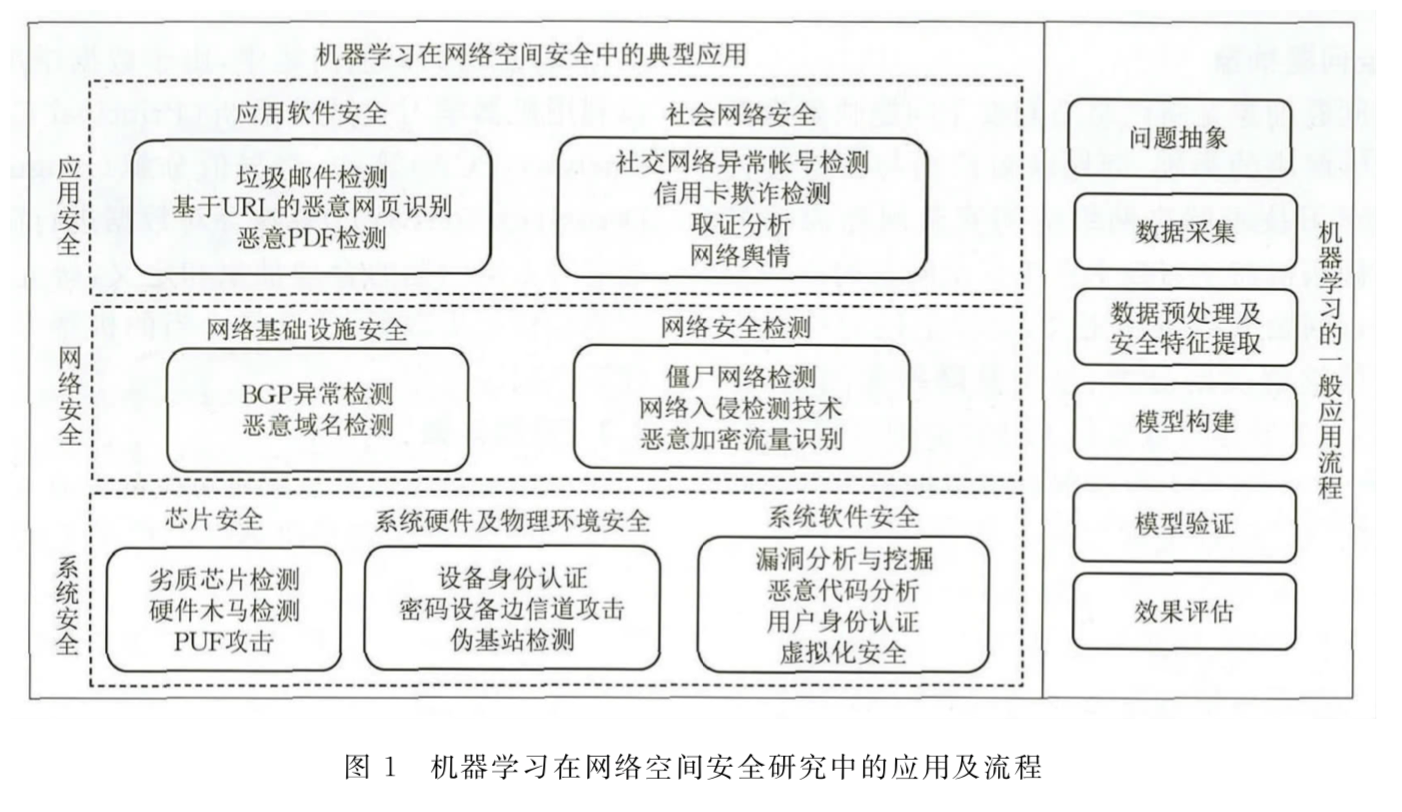
\includegraphics[scale=0.5]{picture/001.png}
        \caption{机器学习在网络空间安全研究中的应用及流程}
        \label{fig:001}
    \end{figure}
  	\begin{figure}[ht]
        \centering
        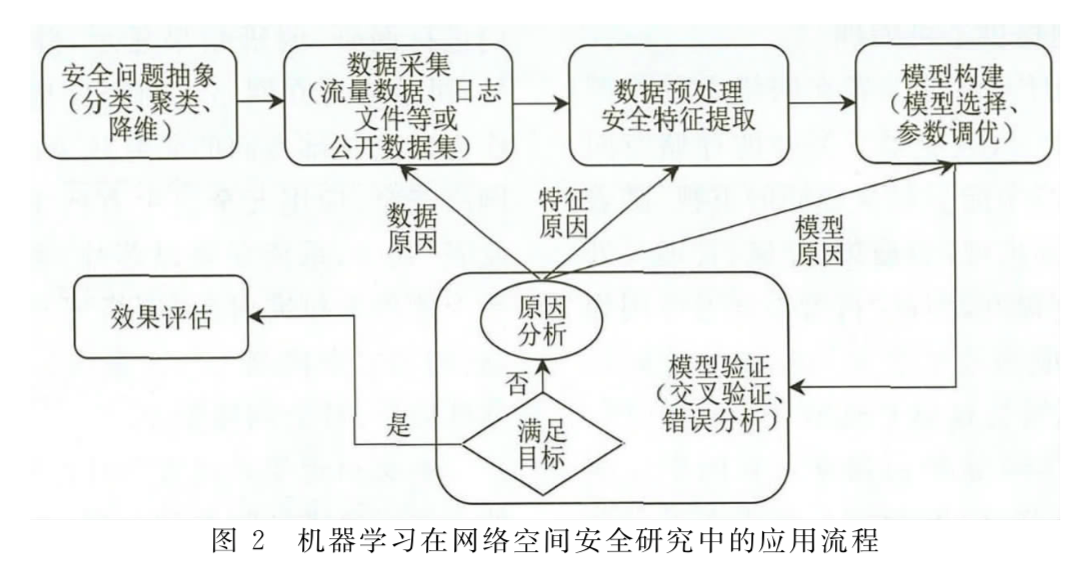
\includegraphics[scale=0.5]{picture/002.png}
        \caption{机器学习在网络空间安全研究中的应用流程}
        \label{fig:002}
    \end{figure}
	\subsection{安全问题抽象}
	安全问题抽象是将网络空间安全问题映射为机器学习能够解决的类别。
	\begin{figure}[ht]
        \centering
        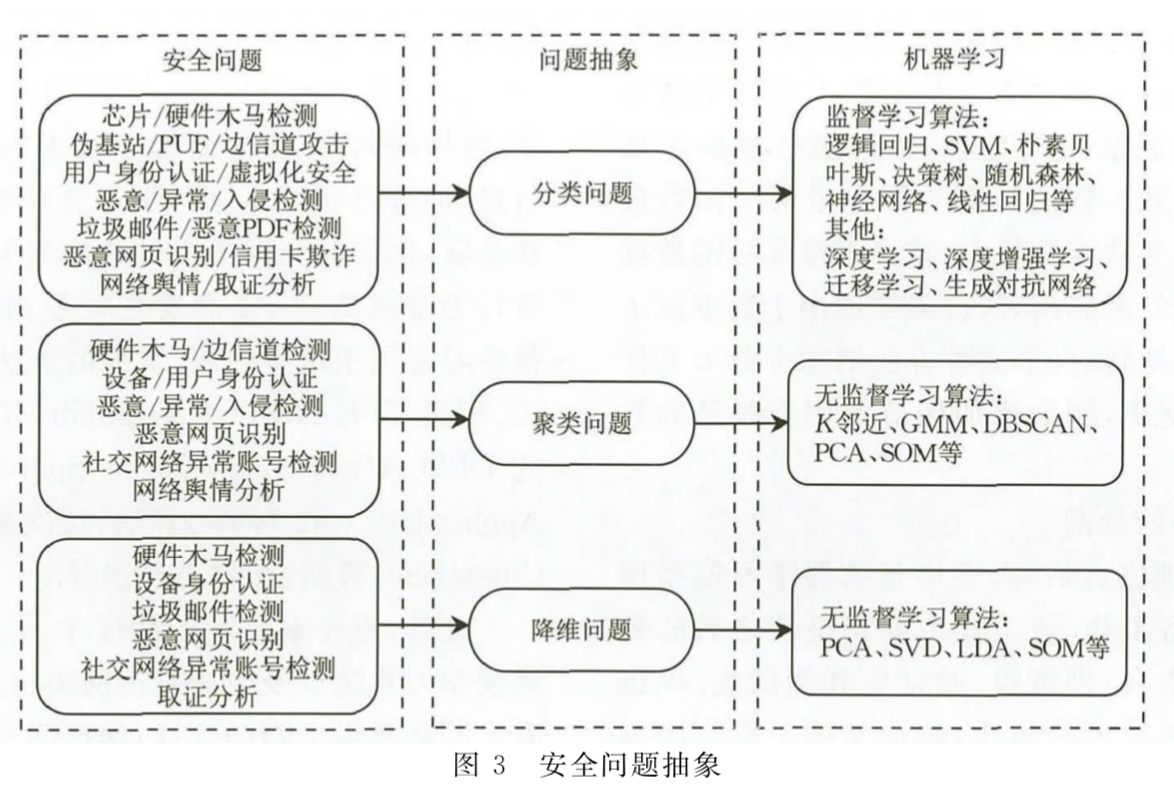
\includegraphics[scale=0.5]{picture/003.png}
        \caption{安全问题抽象}
        \label{fig:003}
    \end{figure}
    \subsection{数据采集}
	自行采集数据和公开数据集
	\begin{figure}[ht]
        \centering
        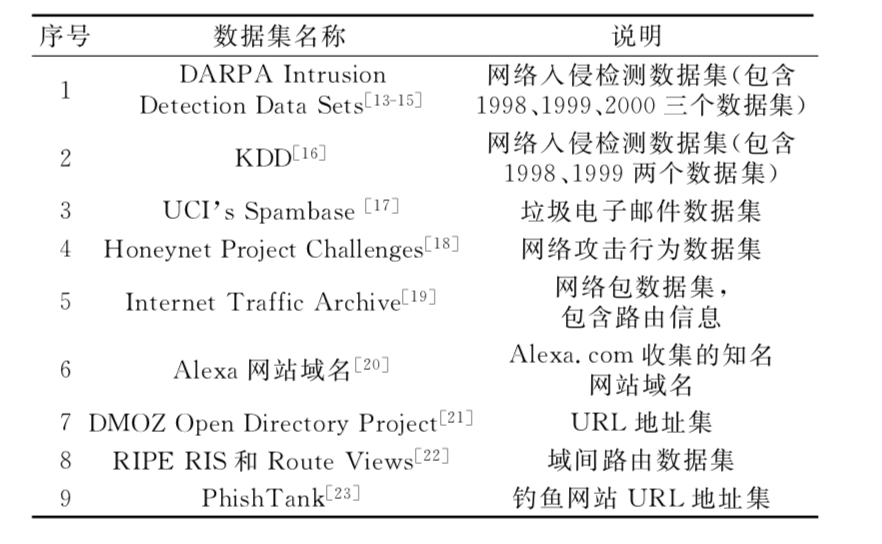
\includegraphics[scale=0.5]{picture/004.png}
        \caption{数据集}
        \label{fig:004}
    \end{figure}
    \subsection{数据预处理及特征提取}
	\subsubsection{数据预处理}
	分析统计数据,对缺失值、异常值、重复值、噪音数据等进行清洗,清洗之后对数据进行归一化操作。
	\subsubsection{数据缺失处理及异常值的处理}
	采集数据集中某个特征缺失值较多时,通常会将该特征舍弃,否则可能会产生较大的噪声,影响机器学习模型的效果.当某个特征的缺失值较少时,可用采用固定值填充、均值填充、中位数填充、上下数据填充、插值法填充或者随机数填充等方法。
	\subsubsection{非平衡数据的处理}
	异常数据样本或恶意数据样本远远少于正常样本时,直接使用机器学习算法构建检测模型效果不佳。为了解决非平衡数据问题,通常使用过采样或欠采样方法构造平衡数据集。
	\subsubsection{数据集分割}
	将整理之后的数据集分为三个集合:训练集、验证集和测试集。训练集用于机器学习模型的构建,验证集用于验证模型及参数调优,测试集用于评估模型在实际使用中的泛化能力。
	\subsubsection{特征提取}
	根据数据预处理后的数据集及目标问题类型,在本阶段选择合适的学习算法,构建求解问题模型,包括算法选择和参数调优。
	深度学习凭借强大的自动提取特征的能力,被用于解决异常协议检测、恶意软件检测、网络入侵检测、BGP异常路由检测以及差分隐私保护等安全问题。(此部分知识欠缺,需继续学习各类算法及适合解决的问题类型)
	\subsubsection{模型验证}
	评估训练的模型是否足够有效,常用k倍交叉验证法。
	\subsubsection{效果评估}
	\begin{itemize}
	\item[*] 分类问题评估指标:正确率、查准率(精度)和查全率(又称召回率)
	\item[*] 异常检测、入侵检测评估指标:误报率、漏报率
	\item[*] 认证领域评估指标:误识率、拒识率
	\item[*] 聚类问题评估指标:一类是将聚类结果与某个参考模型进行比较;另一类是直接考察聚类结果而不利用任何参考模型
	\end{itemize}
	\section{机器学习在系统安全研究中的应用}\label{sec:disanjie}
	对用户身份认证详细记录一下:在基于机器学习的用户身份认证研究方面,主要有利用机器学习攻击传统用户身份认证方法和利用机器学习设计新的用户身份认证机制两个研究点。
	\begin{figure}[ht]
        \centering
        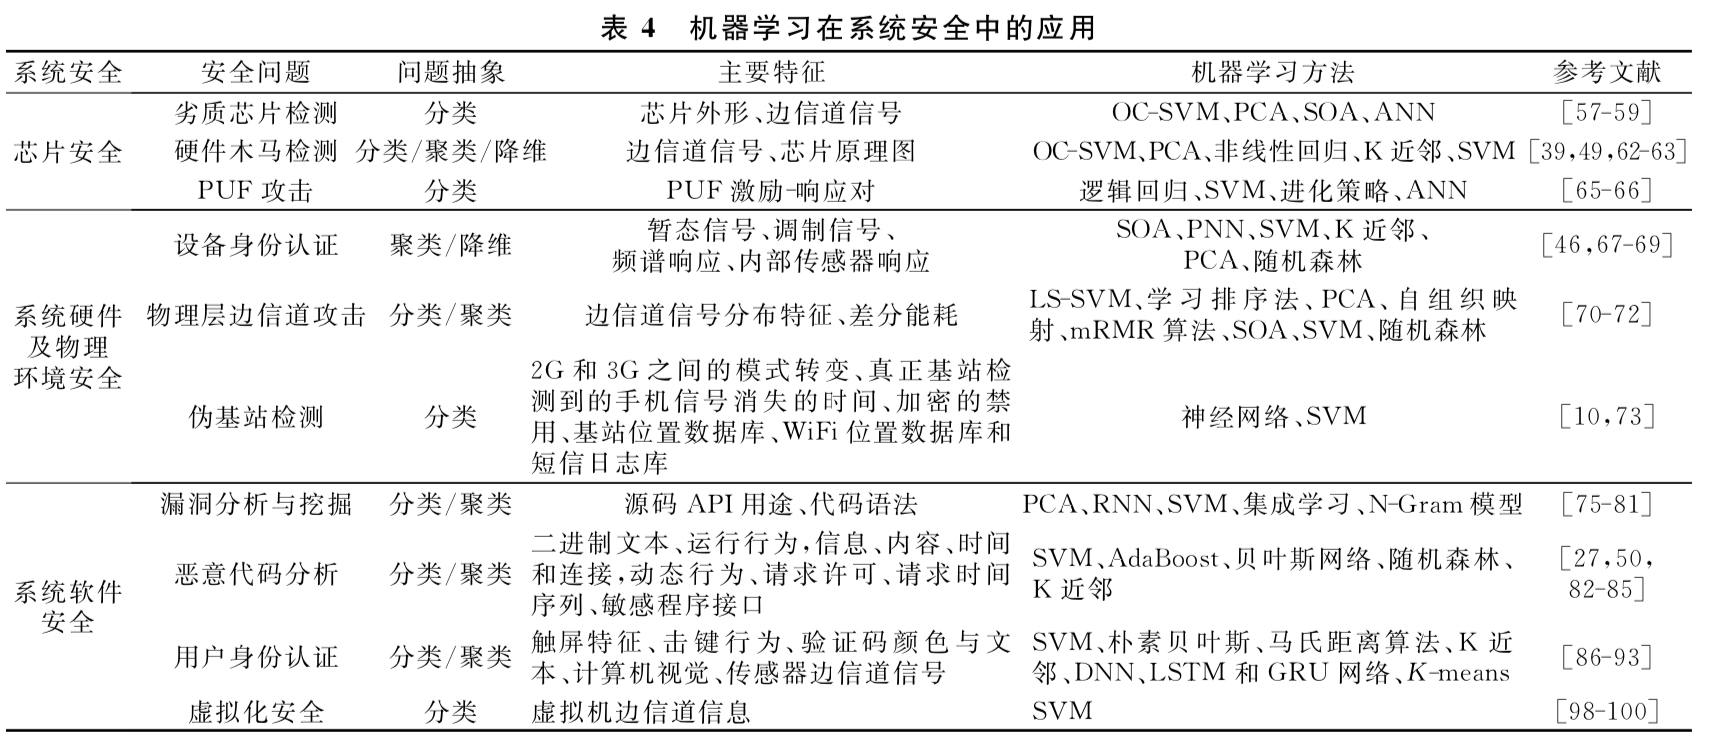
\includegraphics[scale=0.5]{picture/005.png}
        \caption{机器学习在系统安全中的应用}
        \label{fig:005}
    \end{figure}
    \begin{figure}[ht]
        \centering
        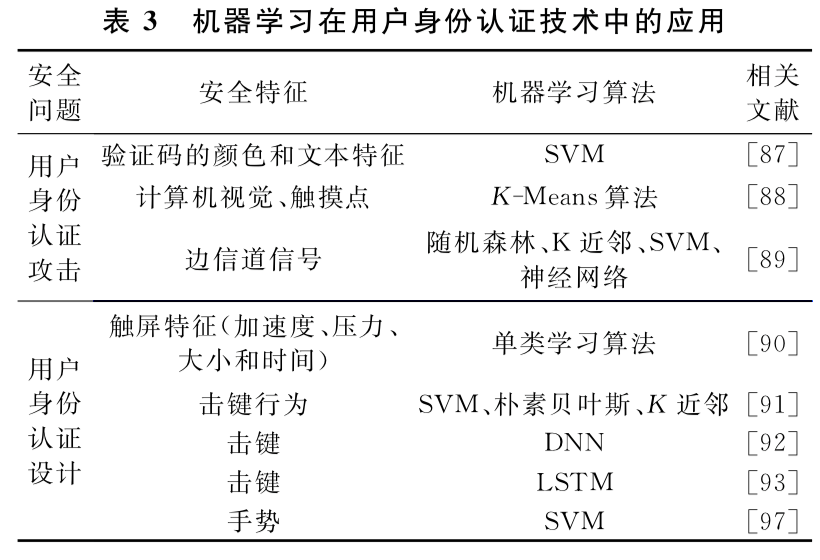
\includegraphics[scale=0.5]{picture/006.png}
        \caption{机器学习在用户身份认证技术中的应用}
        \label{fig:006}
    \end{figure}
	\clearpage
	\section{机器学习在网络安全研究中的应用}\label{sec:disijie}
	对于恶意加密流量识别详细记录一下文中提要的已有研究:《Identifying encrypted malware trafic with contextual flow data》(Procedings of the ACM Workshop on Security and Artificial Intel ligence, 2016)在不解密网络流量的情况下,利用机器学习技术从加密的网络流量中识别出具有恶意行为的网络流量。首先采集了百万级的正常流量和恶意流量,然后分析了TLS流、DNS流和HTTP流的不同之处,具体包括未加密TLS握手信息、TLS流中与目的IP地址相关的DNS响应信息、相同源IP地址5min窗口内的HTTP流的头部信息;然后从上述信息中提取特征,将该特征采用零均值和单位方差进行归一化处理,随后利用L1逻辑回归分类器获得检测模型最优权值,并采用10倍交叉验证进行模型验证。
	《Analyzing android encrypted network trafic to identify user actions》(IEEE Transactions on Information Forensics and Security, 2015)利用机器学习技术分析网络加密流量,用于识别移动终端用户的行为。利用已知APP在移动终端生成网络流量,在网络侧截取网络流量,将网络流的时间序列进行标记,生成有标签的训练集;然后使用层次聚类算法将网络流进行聚类,相似的流被分组在同一个簇中代表有相似的用户行为,不同的流分组至不同的簇;利用整数形式表示每个簇的特征,再使用随机森林算法执行分类操作,将未知的流量分类至不同的流簇中。
	\begin{figure}[ht]
        \centering
        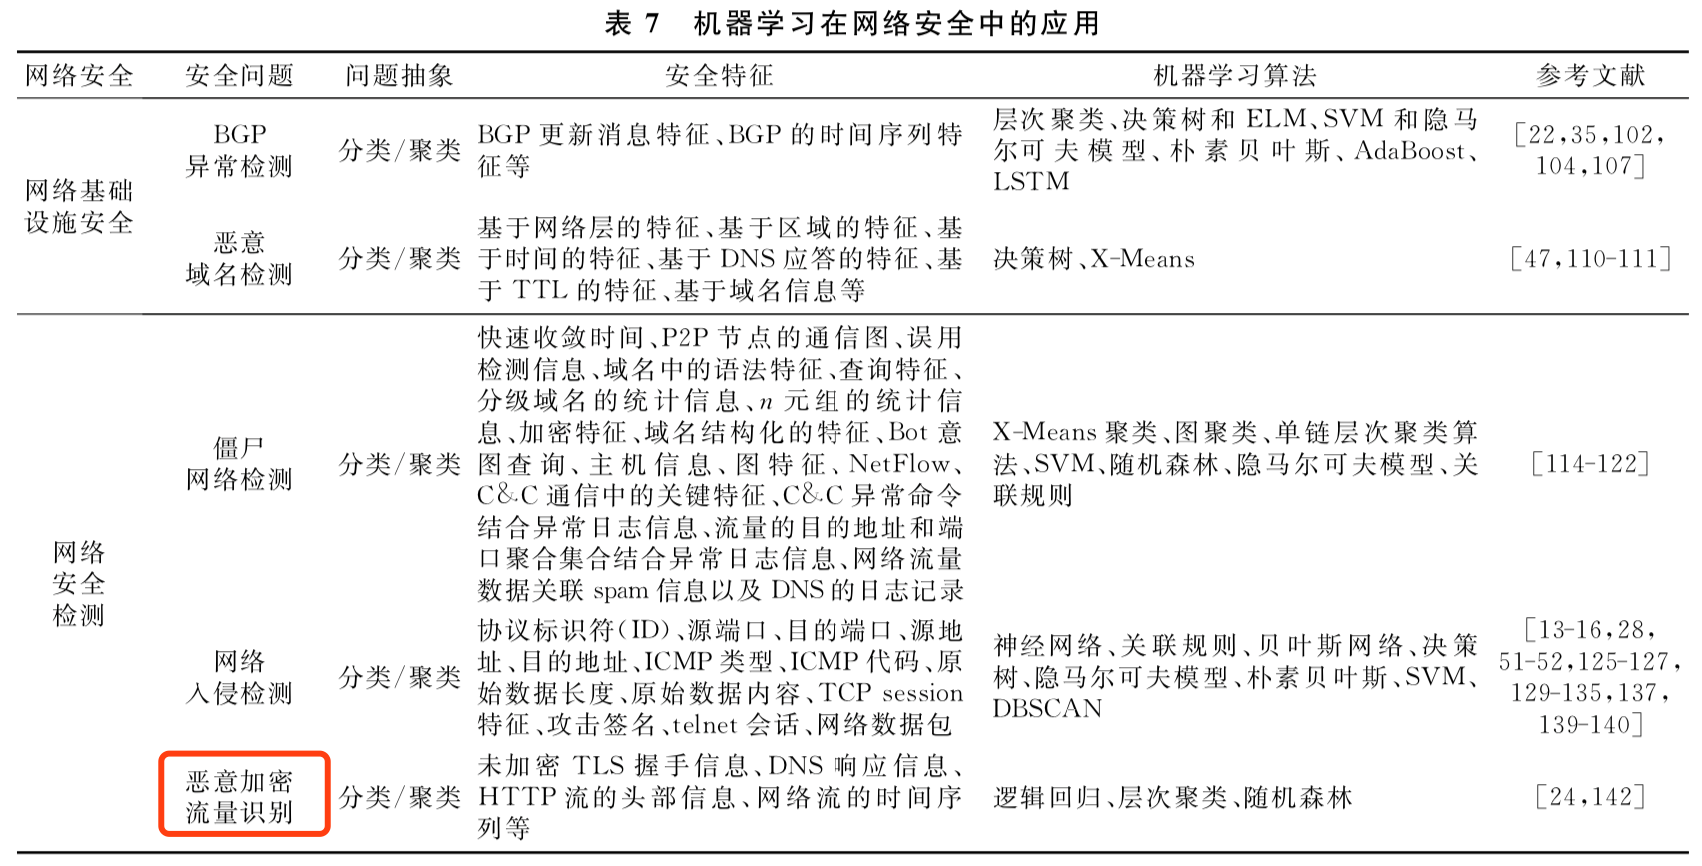
\includegraphics[scale=0.5]{picture/007.png}
        \caption{机器学习在网络安全中的应用}
        \label{fig:007}
    \end{figure}
	\clearpage
	\section{机器学习在应用安全研究中的应用}\label{sec:diwujie}
	\subsection{应用软件安全}
	\begin{itemize}
	\item[*] 垃圾邮件检测(已有过滤技术已趋于稳定)
	\item[*] 基于url的恶意网页识别(基于分类的恶意网页识别和基于聚类的恶网页识别)
	\item[*]  恶意pdf检测(PDF文档的检测研究大多采用PDF文档内容或结构为特征,利用随机森林、SVM、决策树等分类器构建PDF检测器)
	\end{itemize}
	\subsection{社会网络安全}
		\begin{figure}[ht]
        \centering
        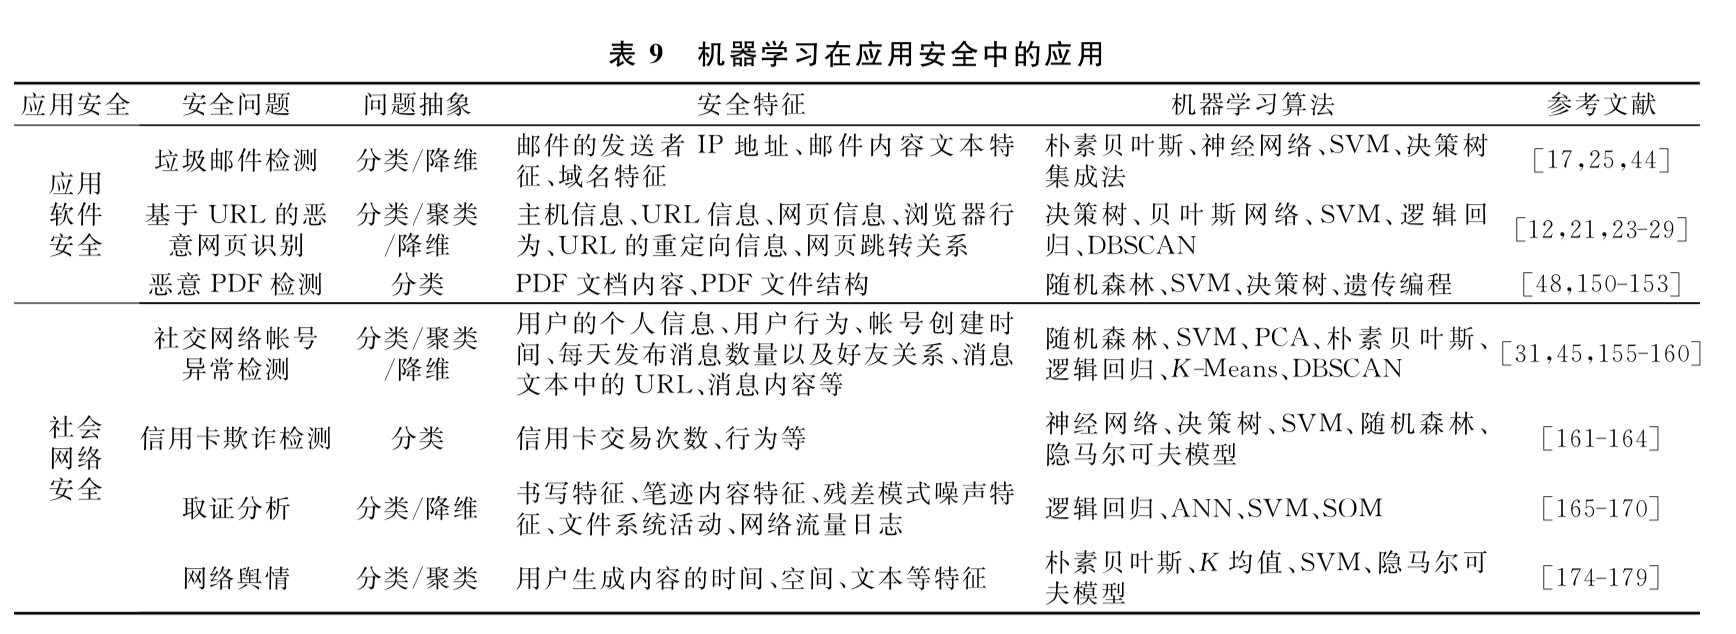
\includegraphics[scale=0.5]{picture/008.png}
        \caption{机器学习在应用软件安全中的应用}
        \label{fig:008}
    \end{figure}
    \begin{figure}[ht]
        \centering
        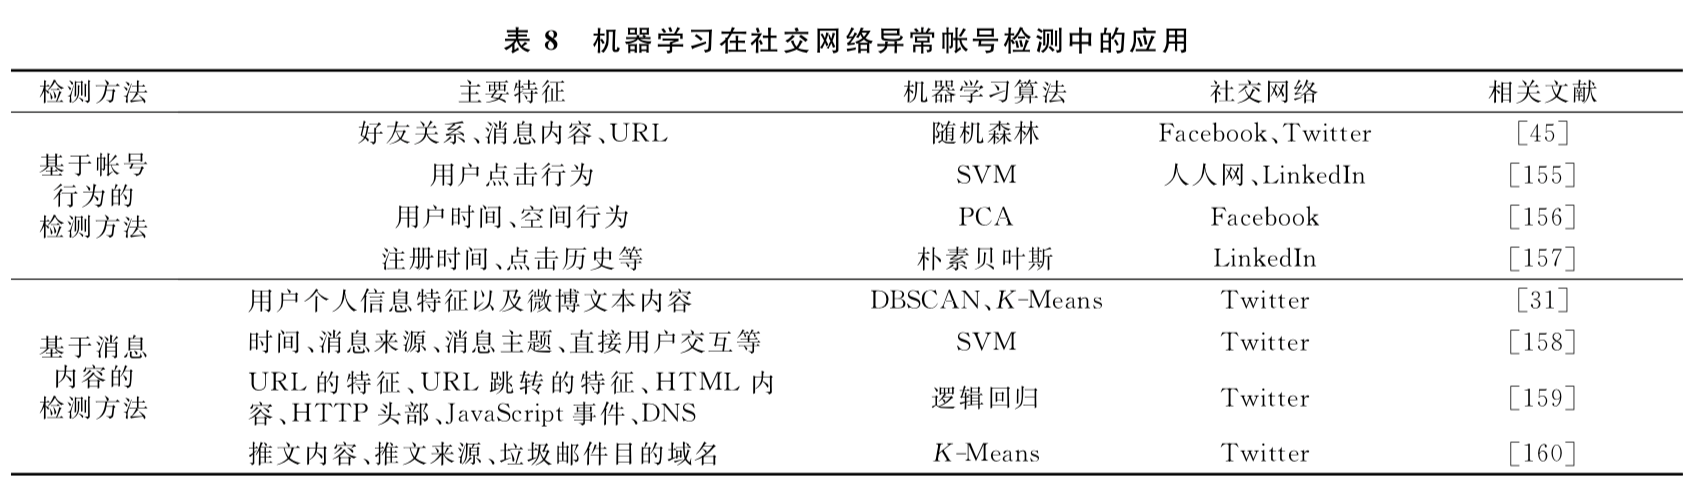
\includegraphics[scale=0.5]{picture/009.png}
        \caption{机器学习在社交网路异常账号监测中的应用}
        \label{fig:009}
    \end{figure}
	\clearpage
	\section{研究展望与挑战}\label{sec:diwujie}
	\subsection{已有技术解决方案在模型的泛化能力、检测准确度、实时性上的能力提升}
	\subsection{机器学习自身难点}
	\begin{itemize}
	\item[*] 如何能够使机器学习的解决方案具备可解释性、鲁棒性 
	\item[*] 如何能够提高实时监测效率以及解决基于机器学习技术的攻击 
	\item[*] 机器学习自身安全(用户隐私、输入样本攻击)
	\end{itemize}
	\clearpage
	\section{个人阅读小结}\label{sec:diwujie}
	\begin{itemize}
	\item[1] 机器学习在网络安全方面能解决问题的能力有限,确定研究方向时需要深入调研,综合考虑研究意义、机器学习对具体问题的解决能力、数据获取等方面。
	\item[2] 初步对恶意加密流量识别比较感兴趣,后续继续阅读相关文献进行总结
	\end{itemize}
	\clearpage
	\bibliography{test}
\end{document}

